\documentclass[a4paper,titlepage]{article}
\usepackage{frontespizio}
\usepackage[english]{babel}
\usepackage[utf8]{inputenc}

\usepackage[a4paper, total={6in, 9in}]{geometry}



\begin{document}
\begin{frontespizio}
\Universita{Verona}
\Dipartimento{Informatica}
\Corso[Laurea]{Informatica}
\Titoletto{Software Engineering}
\Titolo{Second project report}

\Candidato[VR363021]{Giovanni Liboni}
\Candidato[VR359169]{Enrico Giordano}
\Candidato[VR359129]{Alberto Marini}
\Candidato[VR359333]{Alessandro Falda}

\Annoaccademico{2013-2014}
\end{frontespizio}

\tableofcontents

\newpage

\part{Introduction}

This project implements an asynchronous system consists in three principal parts:

\begin{enumerate}

\item a station, that controls velocity of cars;

\item some automatic cars, that set their velocity randomly during the ride and set the ideal velocity thanks to the station;

\item some manual cars, that set their velocity randomly during the ride and receive ``break'' message (but they are not obliged to slow down).

\end{enumerate}

During the execution, is istantiated 50 manual cars and 40 automatic cars and change the speed of each car randomly during the runtime. After a simple ride, the cars decide randomly if they will be exit or not.

\newpage

\part{Graphical interface}

The graphical interface is built with \textit{swing} Java library and consists in two JFrame called ``WallGraphic'' and ``DebugInterface''. The first interface (WallGraphic) is a representation of the situation, composed by a station, some automatic cars and some manual cars. The second interface (DebugInterface) is a textual console that show the program flow, cars display and state and station state. This interface has three option:

\begin{figure}[!h]
\centering
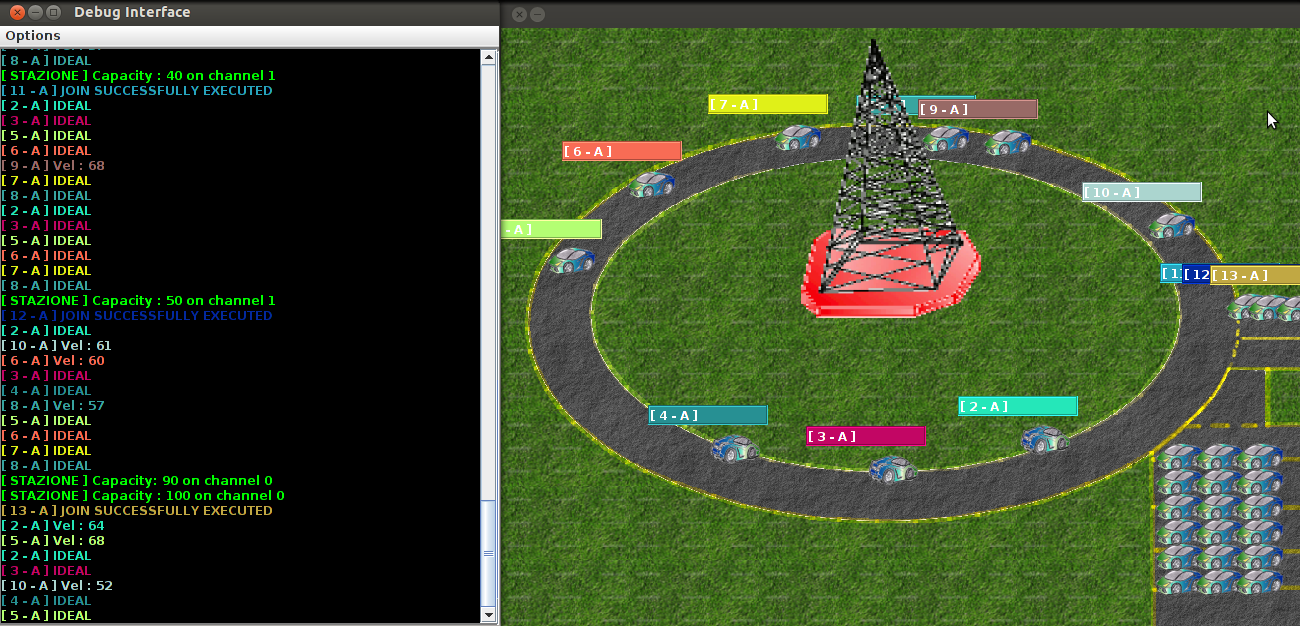
\includegraphics[scale=0.3]{screen.png}
\caption{ScreenShot}
\end{figure}

\begin {enumerate}

\item ``pause'', that stops the program flow acquisition;

\item ``resume'', that resume the program flow acquisition (and enable autoscroll);

\item ``watch'', that disable or enable the autoscroll of the scrollbar.    

\end{enumerate}

Only 200 rows are shown in the screen; after 200 rows, DebugInterface clean itself and delete old rows. This was made because after 200 setText in the same JLabel probably will crash the program.

This is composed by a JFrame that contains a JPanel that contains a JLabel with a black background and a text that was updated by station and cars display.

~

WallGraphic is composed by a JFrame that contains a JPanel with a ``wallpaper'' (the circuit). This JPanel contains in different levels (Z ordered) a station (that is a JLabel with an image) and some cars (that are a JLabels with an image). The cars move theirself in asynchronous way into the ride in 10 different direction (in order to approximate the elliptical path).

The car label have a superior JLabel that contains its id and the car type: the ``M'' letter represent the ``Manual car'' and the ``A'' letter represent the ``Automatic car''. When a car change its direction (X orientation), it changes its image.

\begin{figure}[!ht]
\centering
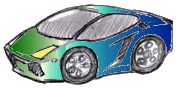
\includegraphics[scale=0.2]{../car.png}
\caption{car label}
\end{figure}


\begin{figure}[!ht]
\centering
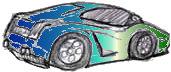
\includegraphics[scale=0.2]{../car2.png}
\caption{car label (different orientation)}
\end{figure}

\begin{figure}[!ht]
\centering

\includegraphics[scale=0.5]{../radio.png}
\caption{station label}
\end{figure}


Every car is a graphical thread that execute the move() method in order to move itself during the ride; when a car exit to the circuit, the thread dead. The velocity is graphically represented by a thread sleep during the movement.

~

This is the Z order of the JLabel:

~

~ ~ ~ ~ ~-1: background image;

~

~ ~ ~ ~ ~ 0: station;

~

~ ~ ~ ~ ~-1: cars;

~

In this way, the cars will pass graphically behind the station and on the background image.


In the park, there is a lot of ``dead car'' that simply occupies the park. This was made because is a graphical strategy to fill a space that may seem empty or messy.

~

The graphical class are contained in the \textit{``graphics''} package.

\section{Design pattern for graphical interface}

Every class of this project must use theese graphical interface, so it was implement a \textbf{Façade pattern}. In fact there is a general class, ``ScenarioGraphic'', that include in itself every graphical istance; in this way, when a class must use a graphical istante, simply call the ScenarioGraphic methods and ScenarioGraphic can modify the graphical istances. 
\newpage
\begin{figure}[!ht]
\centering
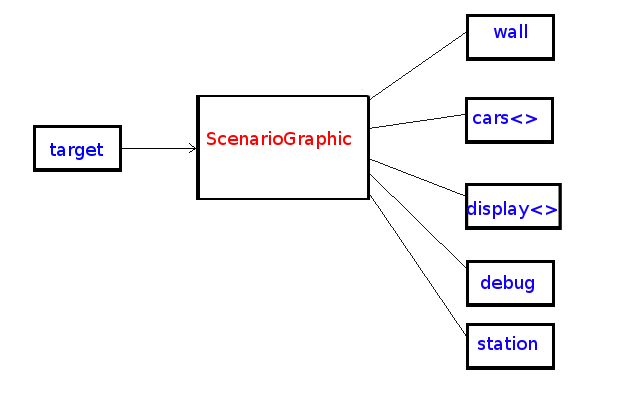
\includegraphics[scale=0.4]{facade.png}
\caption{Façade pattern}
\end{figure}

\newpage

\section{Swing bug}

The Swing graphical library is a simple and usefull library for java application, but in this project it was used at the limit of its potential. So, every car has two graphic threads that work asynchronously with a fast refresh (20 milliseconds). So, during the execution the GUI may be throws this exception: 

\begin{verbatim}
Exception in thread "Thread-1" java.lang.NullPointerException
	at javax.swing.BufferStrategyPaintManager.flushAccumulatedRegion
	...
\end{verbatim}

This is a bug of Swing library of the management of asynchronous threads that have a very high refresh. But is not important for the program execution, simply is rarely thrown this exception.

\newpage

\part{AutoCar and ManCar Classes}

%Queste classi sono delle implementazioni delle interfacce di tipo Runnable e InterfaceAutoCar (e il rispettivo InterfaceManCar) per questi motivi: 
These classes are implementations of Runnable and InterfaceAutoCar interfaces (and the respective InterfaceManCar) for these reason:

\begin {itemize}

\item contain a method \begin{verbatim} public void run() \end{verbatim} which represents what each machine must do from the point of view of the movement (i.e. run the route in the circuit);
%\item contengono un metodo \begin{verbatim} public void run() \end{verbatim} che rappresenta ciò che ogni macchina deve fare dal punto di vista del movimento (cioè eseguire il tragitto nel circuito);

%\item implementano le corrispettive classi della loro interfaccia.
\item implement the corresponding classes of their interface.

\end {itemize}

%Il fatto di implementare due interfacce differenti è stato utile per rappresentare un comportamento diverso come da specifiche per il messaggio di ``break'' ricevuto dalla stazione e in particolar modo per utilizzare il design pattern di tipo \textbf{Adapter}. Infatti avendo due implementazioni differenti, per utilizzare diversamente un metodo non è possibile fare un Override e quindi bisogna appoggiarsi ad una classe intermedia (AdapterAutoToManual) che estende la classe chiamante ma implementa la classe da cui si vuole ereditare il comportamento.   
Implement two different interfaces is useful to represent a different behavior for the ``break'' message received from the station and in particular for using \textbf{Adapter} design patterns type. In fact, to use a different method you can not make an override and so you have to rely on a intermediate class (called AdapterAutoToManual) that extends the calling class but implements the class which you want to inherit the behavior.

%Quindi di fatto esistono due interfacce distinte di AutoCar e ManCar che vengono implementate dalle rispettive classi e che hanno comportamenti differenti; se si vuole utilizzare la AutoCar come ManCar bisogna istanziare la classe AdapterAutoToManual e utilizzare tramite essa i metodi della classe ManCar. 
So in fact there are two distinct interfaces to AutoCar and Mancar that are implemented by the respective classes and have different behaviors; if you want to use the AutoCar as a ManCar you must instantiate the AdapterAutoToManual class and use through it the ManCar class methods.

\begin{figure}[!ht]
\centering
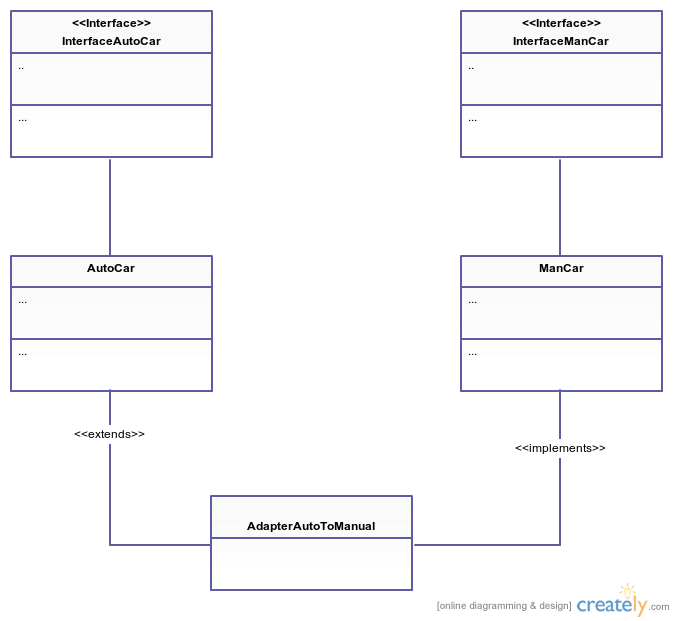
\includegraphics[scale=0.4]{adapter.png}
\caption{Adapter pattern}
\end{figure}


\newpage

%Per rendere possibile l'utilizzo della propria parte grafica da parte della classe AutoCar e ManCar, è stato fatto in modo che questa classe istanziasse dentro di essa l' istanza grafica ``CarGraphic'', in modo da avere pieno controllo sulla propria parte grafica. 
To make possible the use of graphics part by AutoCar and ManCar classes, this class can instantiate in it the ``CarGraphic'' graphics instance, to have full control over their graphics part.

%Questo è stato utile per gestire il movimento delle macchine in maniera asincrona rispetto alle altre macchine ma anche all'esecuzione del programma. Inoltre in questo modo anche alla classe ScenarioGraphic è permesso di avere controllo del comportamento e della parte grafica sia delle AutoCar sia delle ManCar; istanziando infatti la classe AutoCar o ManCar, si crea in automatico l'istanza grafica, quindi è possibile gestirla facendo accesso alle singole istanze delle loro classi. 
This was useful for managing the asynchronously machine movements compared the other machines and the execution of the program too. Moreover, in this way is allowed to ScenarioGraphic class to have control of behavior and the graphics parts of both AutoCar and Mancar classes; in fact, by instantiating Mancar or AutoCar class it automatically creates the graphic instance, so you can manage it by accessing the individual instances of their classes.

~

%Questo rende inoltre utile l'utilizzo del \textbf{Façade Pattern}, perché si vuole utilizzare una singola classe per controllare tutte le istanze grafiche (dove è permesso).
This make useful to use \textbf{Façade Pattern}, because you want to use a single class to control all graphics instances (where permitted).

\end{document}

